\chapter{Application Design}

This chapter details with the user interface and design elements of the application, specifically how the application appeared when the user testing took place. It details  the design decisions made and then proceeds to explain and justify why it was thought that making these decisions would improve the user experience. The results of the user testing and whether or not the design worked is detail in chapter .

\section{Category and Experience Selection}

When the user first connects to the web application, they are shown the view in figure \ref{fig:view1}. This view allows them to input their experience with German, as well as selecting the category of article that they wish to read. Four different experience levels are available, "beginner", "intermediate", "advanced" and "near fluent". The decision to categorize language experience this was made for a number of reasons. First and for most, the names of the different experience levels are in English and are commonly used as descriptions of language proficiency. While it would have be possible to use much more formal definitions of language proficiency, for example the Common European Framework of Reference for Language (CEFRL). These definition are not commonly taught and would most likely confuse a large proportion of users. Once "beginner", "intermediate" and "advanced" had been decided upon, the decision was made to add a forth level "near fluent" to distinguish between users  who needed barely any help and users who needed some help. It was also believed that fluent German speakers would have no need to use the application, and therefore did not need to be considered when designing these levels.

\begin{figure}
	\caption[Screenshot of the Category Selection View]{Screenshot of the category selection view, where the user inputs the category of article they want to read, as well as their experience level.}
	\label{fig:view1}
	\begin{center}
	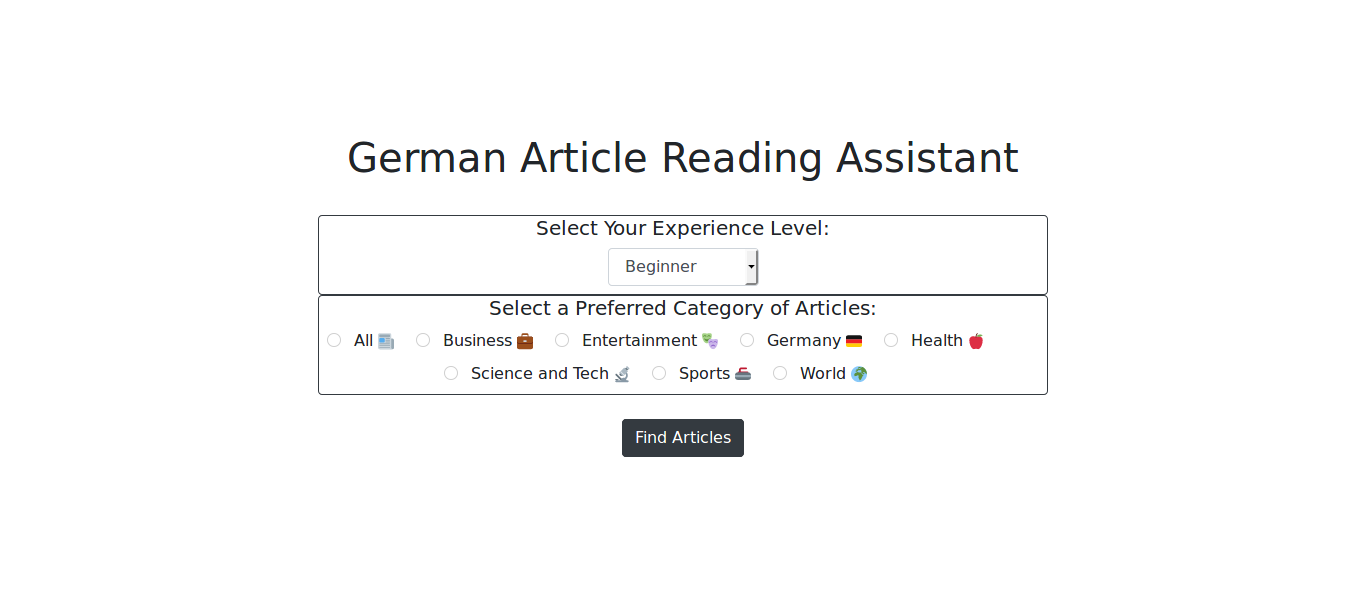
\includegraphics[width=\textwidth]{Graphics/View1}
	\end{center}
\end{figure}

The user then goes on to select a category of article. The Selections available are "All", "Business", "Entertainment", "Germany", "Health", "Science and Tech", "Sports" and "World". These categories were chosen to reflect the traditional new categories that one would find on a news website. The decision was made to use English titles rather than German ones, to allow a range of users to able to understand what the categories are. German titles were used briefly during a stage of development, but were switched to English as it was believed that some users would not be skilled enough in German to understand the meaning of all the titles without access to translations, which are not currently available on this screen. 

A symbol was added next to the name for each category. Primarily to make it easier to identify the categories upon sight, but also to broaden the colour pallet being used in the application.

The initial prototype of the application had a different article selection screen, Where the URL of the desired article was inputted instead of a category selection screen. This had both advantages and disadvantages over the selection model in the final screen. This allowed the user to find articles that interested them and then input them into the application and continue reading there, but it also relied on the user having to be able to find article that interested them externally. Ideally, it would have been best to have both the category selection and direct article input methods implemented, perhaps with different input screens, however, due to time constraints. This was not implemented.

\section{Article Selection}

Once the user has inputted their ability level and desired category of article, they are then presented with the view shown in figure \ref{fig:view2}. This is a list of articles in the selected category, with titles in German, followed by a difficulty rating, also in German. Titles are left in the original German as the level of reading required to read the title is most likely less than the reading level of the user, allowing them to select their own articles. If not, the difficulty ratings (also in German) provide a clear indication of the level of the articles. 

\begin{figure}
	\caption[Screenshot of the Article Selection View]{An example of the article selection view, here the user is shown a list of articles in their selected category as well as the difficulty rating for each article. They then go on to select an article from the list.}
	\label{fig:view2}
	\begin{center}
	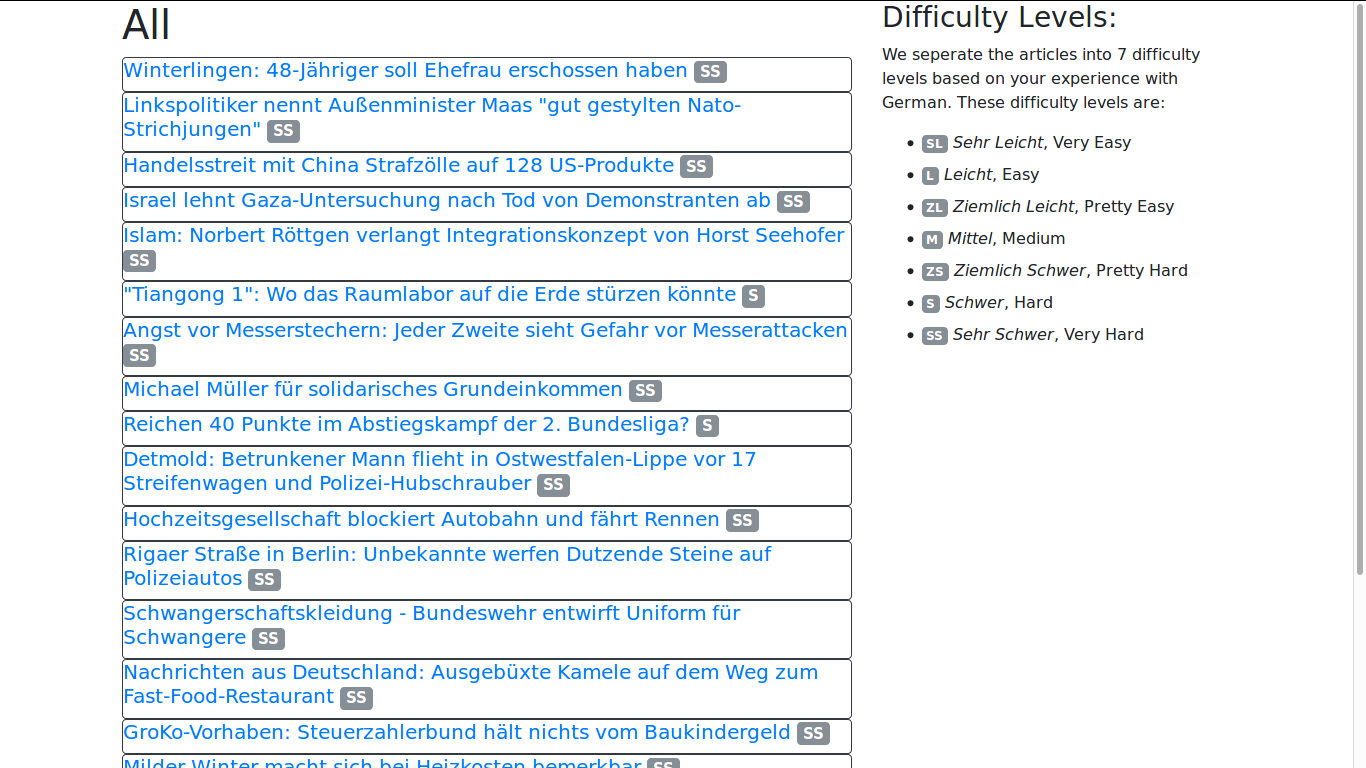
\includegraphics[width=\textwidth]{Graphics/View2}
\end{center}
\end{figure}

To right of the list of articles, in the position where the gloss will be in the article view, a list of definitions of the different difficulty rating can be seen. These, going in order from most difficult to least are "SS", "S", "ZS", "M", "ZL", "L" and "SL". These difficulty ratings were chosen as they are acronyms of German phrases that translate to the appropriate difficult levels, each one of them having a unique initialisation. Seven categories were used, expanding the standard "Easy", "Medium" and "Hard" to include "Very Hard", "Somewhat Hard", "Somewhat Easy" and "Very Easy". These categories can be placed easily on a scale by a user, and then be used to identify with a fair amount  of precision how hard said end user will find the article.

The decision to include the definition box was to make sure that the user could map the German initialisation to the English category definition as no full German words are used in the rating labels and the end user might not be of level where they can perform this mapping without assistance.  

\section{Article Reading}

Once the user has selected an article from the list, they are shown are the view in figure \ref{fig:view3} which is primarily the content of the article. A button to take the user back to list view is shown to left of the article. On the right of the article text, there is a box which prompts the user to click on words. An additional visual prompt is provided, the cursor changes to the common "pointer" cursor when over a word in the article, suggesting that the word can be clicked on.


\begin{figure}
	\caption[Screenshot of the Article Reading View]{The article reading view, where the user can read the contents of their selected article. To the left of the article content is a button taking them back to article selection view and to the right is the gloss column, which contains a prompt telling the user click on articles. }
	\label{fig:view3}
	\begin{center}
	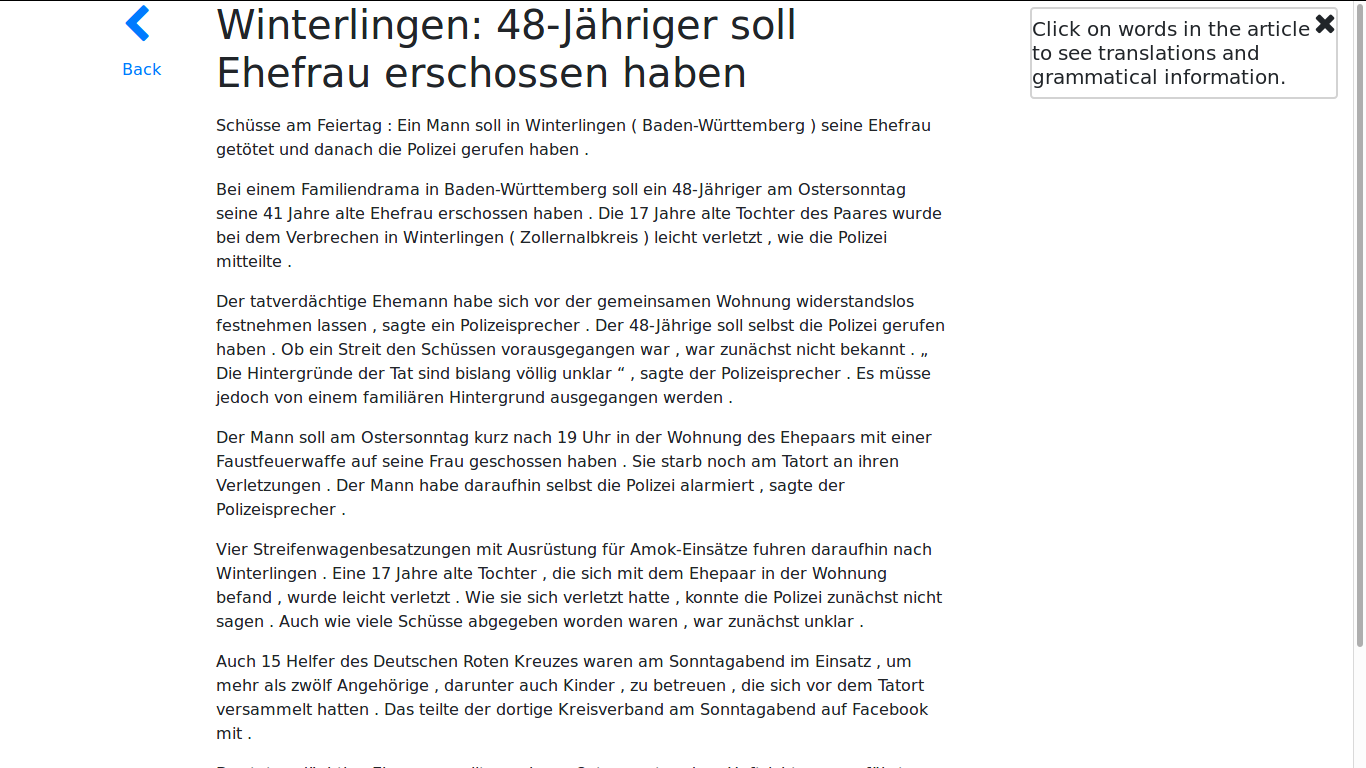
\includegraphics[width=0.7\textwidth]{Graphics/View3}
\end{center}
\end{figure}

Clicking on a word on the article, will make a gloss item to appear on the right of the screen, making the screen appear similar to the view shown in figure \ref{fig:view4}. This position is a marginal gloss, which, is a form a gloss that is effective \autocite{abuseileek2008}. New items appear at the bottom of the column, permanently, until dismissed. If there are too many gloss entries, then a scroll bar will appear, allowing the user to scroll down. These gloss entries are permanent until dismissed to prevent the user from having to lookup the same word multiple times.

\begin{figure}
	\caption[Screenshot of the Article Reading View with Gloss]{Another screenshot of the article reading view, this time with a gloss entry in the margin.}
	\label{fig:view4}
	\begin{center}
	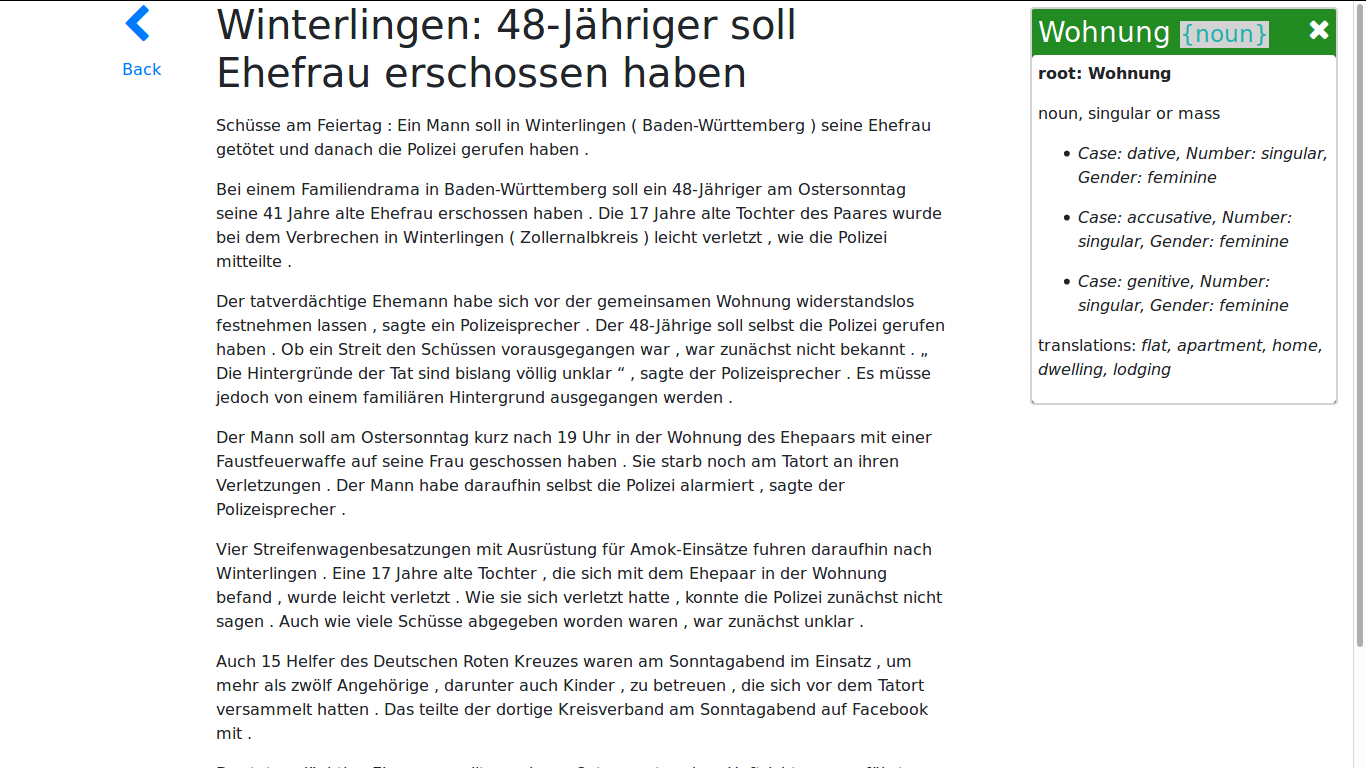
\includegraphics[width=\textwidth]{Graphics/View4}
\end{center}
\end{figure}
 

\subsection{Gloss Items}

\begin{figure}
	\caption{Screenshot of a Gloss Entry}
	\label{fig:gloss}
	\begin{center}
	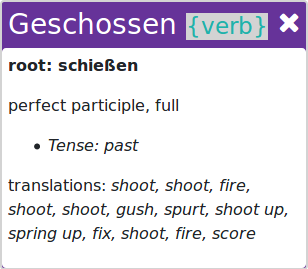
\includegraphics[width=0.3\textwidth]{Graphics/Gloss}
\end{center}
\end{figure}

The design of the gloss items was inspired by the look of the standard dictionary entry, an example of the design can be seen in figure \ref{fig:gloss}. The top of the gloss is a colour specified by the lexical category of the word; green for nouns, purple for verbs, blue for adjectives, red for any others and black for ones that cannot be identified. The header then contains the form of the words as it appears in the text, followed by the lexical category, in curly brackets, with unique text and background colours. A white cross is on the right of the header, clicking it dismisses the gloss entry, removing it from the gloss. 

The body of the gloss is divided into three parts. The root word, the grammatical information and possible translations of the root. The root is presented at the top, in bold. This is done so that if the user can identify the word by the root, than they only need to read that. 

After the root, the grammatical information of the word. First is a short description of the word's lexical category and form of the word. Following this is a bullet point list of the possible reasons the word has mutated from the root; Its tense and person if it's a verb, gender, plurality, and case if it's a noun and other information for other lexical categories. 

Finally the body is concluded with various translations of the root words \autocite{gettys2001}, including all senses of the word. In the case that the program cannot find a translation, the phrase "no translations found" is presented instead. 
 